\chapter{Architecture}
\label{ch:architecture}




“ This chapter is about architectural styles, application architectures, and architecture patterns. A style describes how to implement a specific architecture, while an architecture pattern explains how to address a specific concern within an architecture but is broader than a design pattern. I suggest you not get too hung up on the differences, but just understand that DDD can reside at the heart of a lot of surrounding architectural influences.”
Excerpt From: Vernon, Vaughn. “Implementing Domain-Driven Design.”

\comment{We need to emphasize that there are many ways of doing architecture and many reason for doing particular architectures. Functional and non-functional requirements}

\section{Monolithic}
The word monolith describes a application that exists as a single unit, having  By having the entire application as a single entity, the source code can be developed and managed together, giving multiple advantages\cite[p.~68]{long2017cloud}. The developers can add functionality on top of the existing code base quite easily, utilizing programming language constructs. Communication can be done internally, between processes, not relying on non-deterministic communication channels working. These immediate advantages begin to fade as the application grows in size. The code base reaches a size where small changes in one part of the application might well incur unforeseen changes in other parts. Centralizing the application decreases risk of failure, but at the same time forces development teams to coordinate changes, making sure breaking changes are not introduced\cite[p.~68]{long2017cloud}. 

According to \citeauthor{fowler2014microservices} enterprise applications often consist of three main parts: client-side user interfaces, shared common database management systems and monolith server-side applications. The server-side application is a large and complex application, packed into a single executable. The application binds interface and database together, executing domain logic basked on user input, retrieving and updating data as needed. A comparison of the monolith and microservice architecture can be seen on Figure \ref{fig:architecture_microservice_definition}, each figure represents a piece of functionality where the monolith has all piecies gathered in a single executable, the microservice approach distribute functionality into independent services.

\begin{figure}[!htb]
  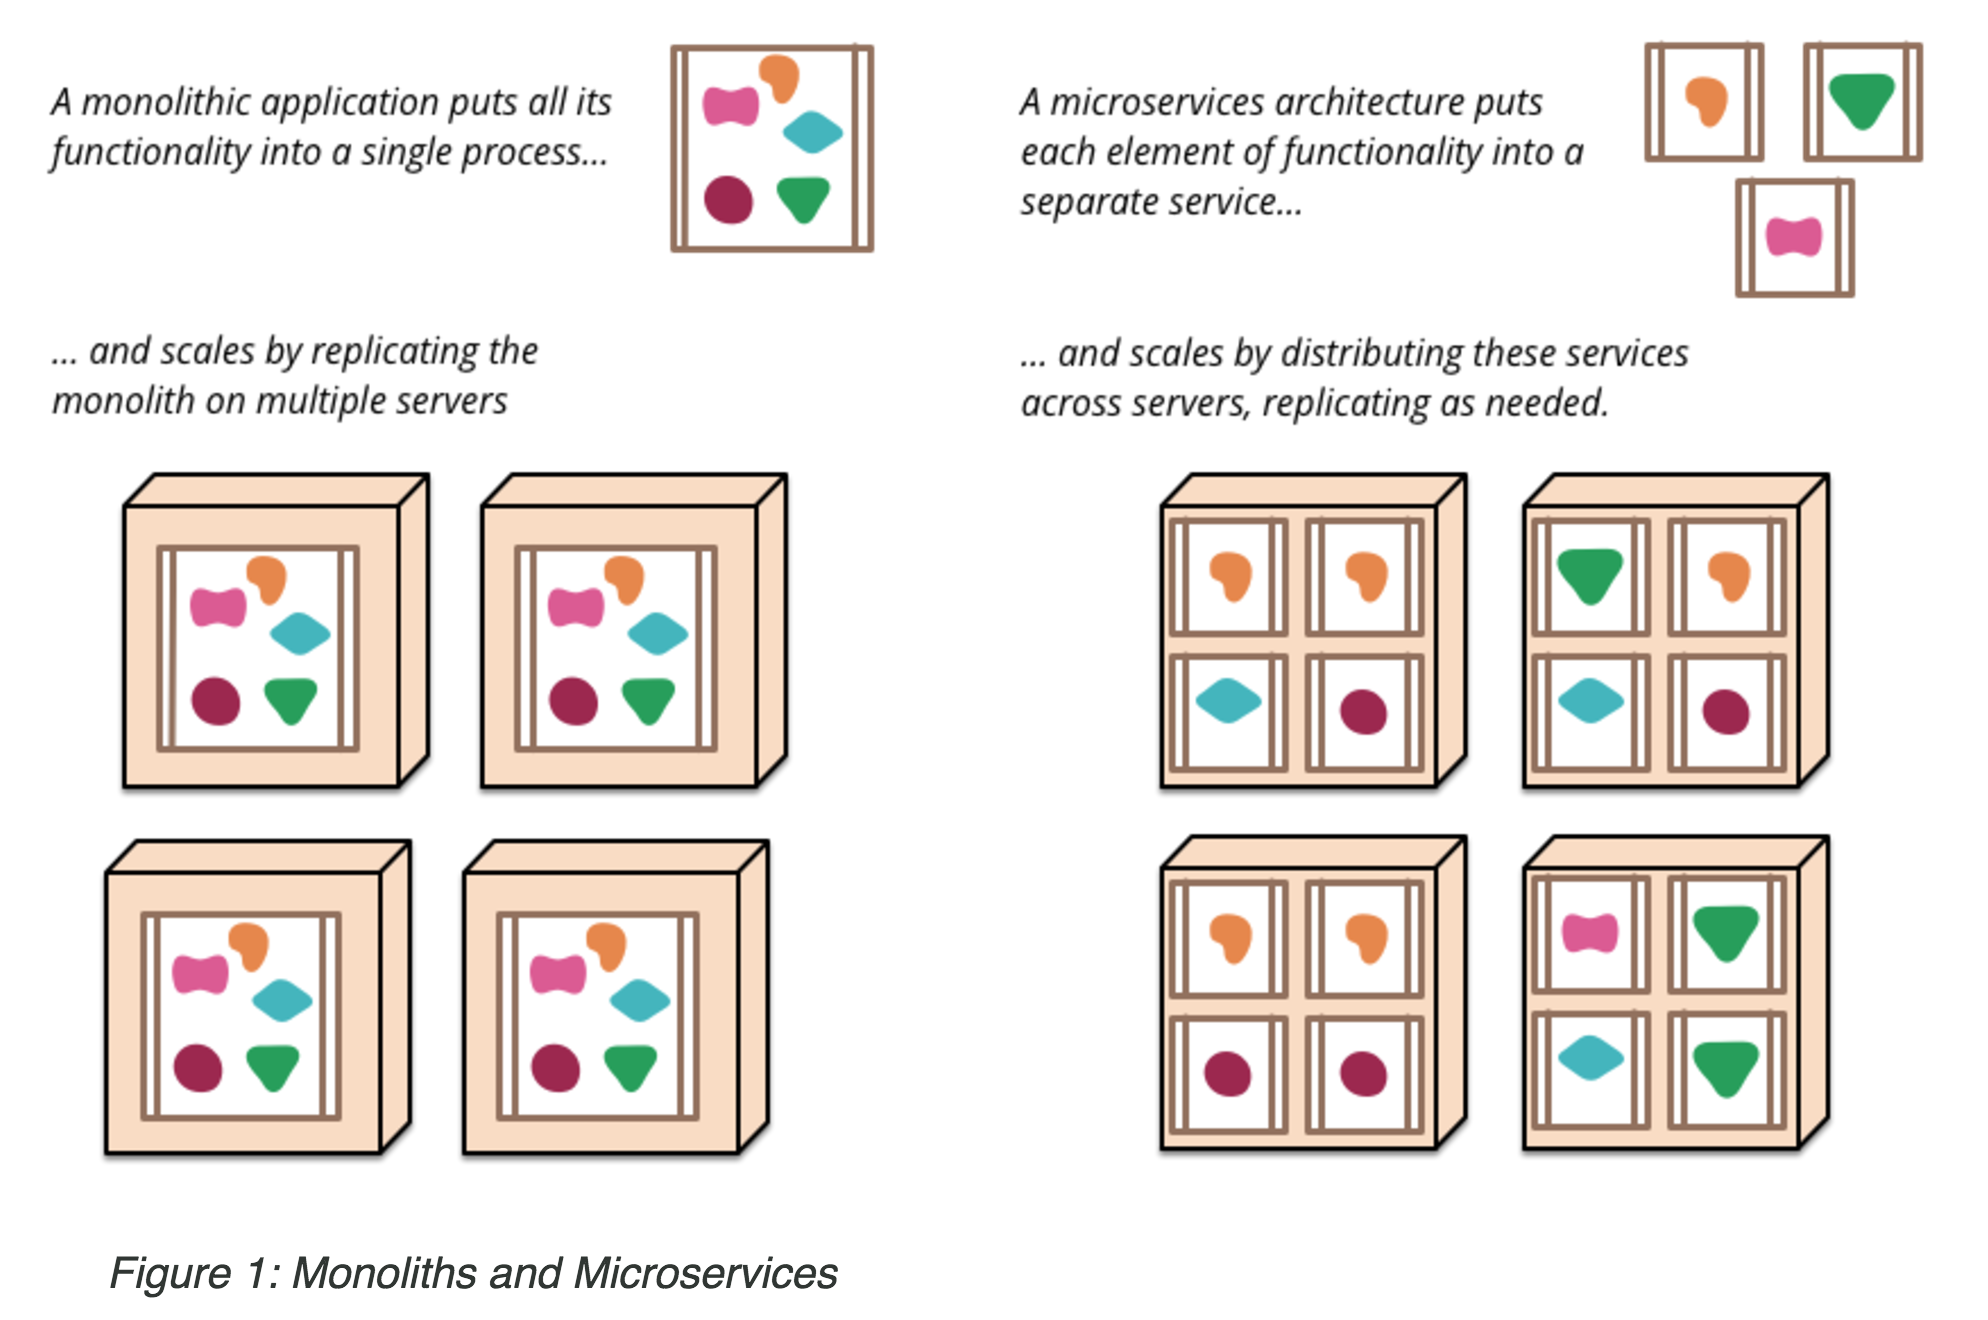
\includegraphics[scale=0.27]{architecture_microservice_definition}  
  \caption{Monolith and Microservice architectures compared}
  \label{fig:architecture_microservice_definition}
\end{figure}


“Chapter Fourteen. Maintaining Model Integrity”\cite{evans2004domain}
Kig på dette kapitel, der er noget om at vedlige holde domæne model, og udfordringerne i at have et stort system.


\note {
The client-side user interface consists of HTML pages, with some underlying javascript files. The database is a shared among all applications in the enterprise, implemented as a relational database, containing tables for the entire business domain. The server-side application is a monolith, binding interface and database together, executing domain logic based on user input and retrieving and updating data as needed. The server-side application is a single executable.

"To start explaining the microservice style it's useful to compare it to the monolithic style: a monolithic application built as a single unit. Enterprise Applications are often built in three main parts: a client-side user interface (consisting of HTML pages and javascript running in a browser on the user's machine) a database (consisting of many tables inserted into a common, and usually relational, database management system), and a server-side application. The server-side application will handle HTTP requests, execute domain logic, retrieve and update data from the database, and select and populate HTML views to be sent to the browser. This server-side application is a monolith - a single logical executable[2]. Any changes to the system involve building and deploying a new version of the server-side application." \cite{fowler2014microservices}
}

\section{Domain Driven Design}
As developers we want to take a complex domain, that is too overwhelming in its natural form, and create a abstraction that allows developers to focus on a subset of the problems. The model transform raw and complex data, making it possible to comprehend the problems and take decisions trying to solve them. Models can help predict problems and take decisions. Models evolve over time, and capture more of the complexity as they evolves\cite{evans2016tackling}.

In Evans terminology a domain consists of a subset of models, with a smaller granularity, only including what is necessary to make decisions about a single problem. In his book Domain Driven Design Tackling Complexity in the Heart of Software\cite{evans2004domain}, Evans state that code should only be based on a single model, and a combination of code based on different models, results in buggy, unreliable code, that is hard to understand. Models need to have a narrow focus on a specific problem within the domain. A model is kept simple by only serving a limit amount of use, which is perfectly fine according to Evans. A simple model is exactly what we are trying to achieve. Models need to be useful relative to a specific problem, meaning that our models of the domain needs to be very small and specific, usable in a specific context. 

Evans uses context as a measure for what underlying understanding there exists of the domain, and which situations the model should be used. The model contains assumptions and is created with outset in the context. It is important to limit the use of a model to the intended context. The context should be reflected in team organization and the code base, only certain parts of the team, code base and database schemas should use the model applied in that context.\cite[p.~335]{evans2004domain}

Evans puts a lot of emphasis on analysing the domain and identifying what he calls bounded contexts. Bounded contexts define the range of each model, which context does it apply to,



"Rigorous  modeling  conventions  must be balanced with free exploration of models in collaboration with non Etechnical people.  Tactics  and  strategy  must  be  combined  to  succeed,  and  DDD  addresses  both  tactical  and  strategic design. " DDD Reference 2015

\section{Service-Oriented architecture}





\begin{figure}[!htb]
  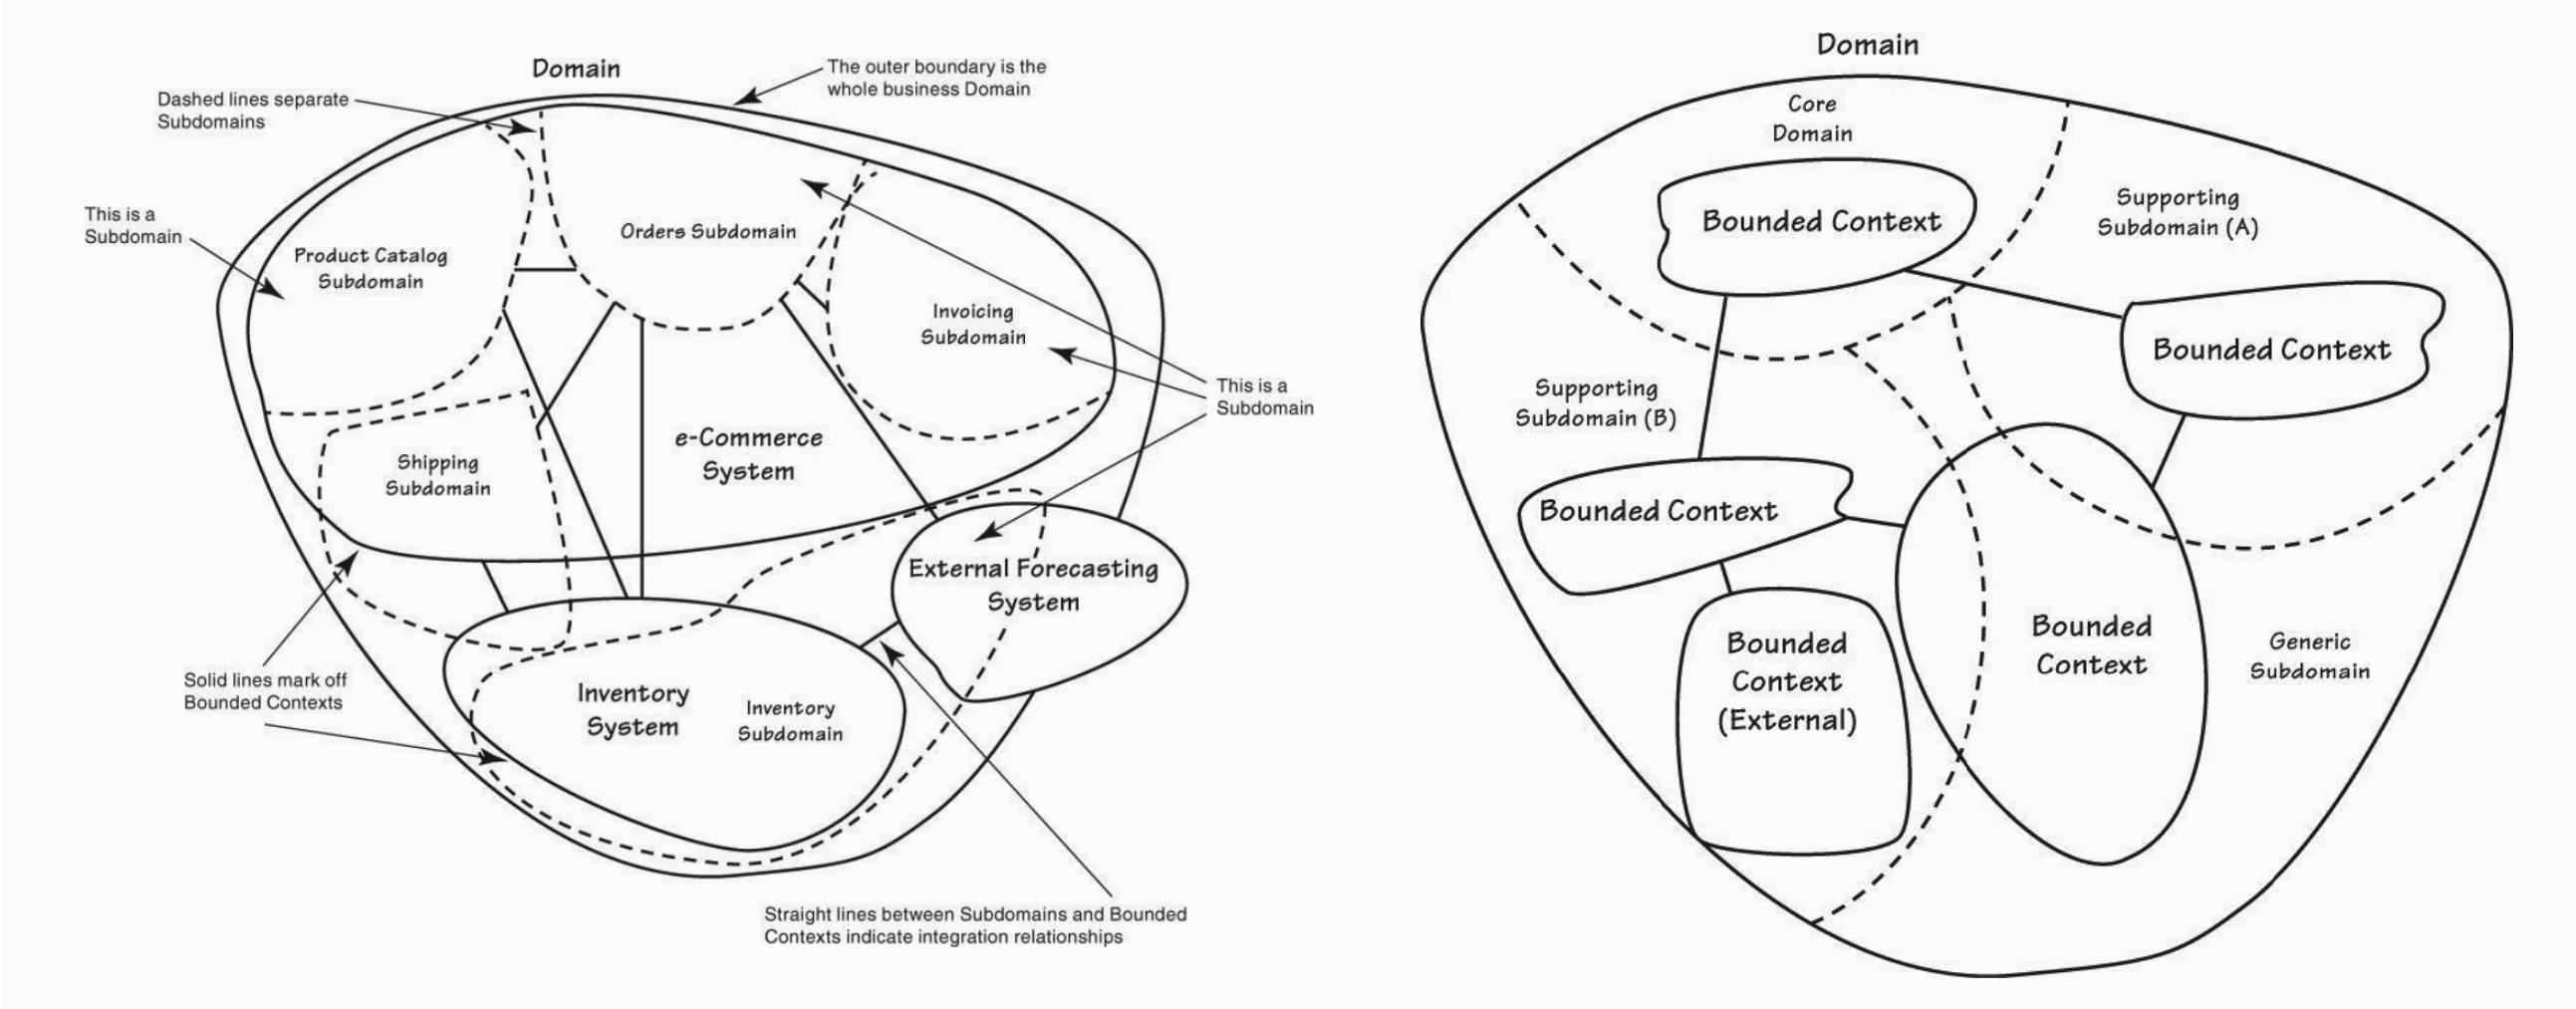
\includegraphics[scale=0.2]{architecture_bounded_context}  
  \caption{A abstract representation of the Danske bank business domain, including Sub-domains and bounded contexts}
  \label{fig:architecture_bounded_context}
\end{figure}

\section{Microservices}
Microservice architecture stems from a mix of SOA and UNIX philosophy, giving a system composed of many small intercommunicating services. Each individual service should have well defined and limited functionality and a well defined interface for external communication. Services communicate with each other through their interfaces and together they achieve a overarching business goal. \citeauthor{morgantini2013whatAreMicroServices} defines microservices as the following:

\begin{quote_highlight}
A system built using micro-services is a system that is built up of small, lightweight services, where each performs a single function. The services are arranged in independently deployable groups and communicate with each other via a well defined interface and work together to provide business value.\cite{morgantini2013whatAreMicroServices}
\end{quote_highlight}

\subsection{Defining characteristics}
\textbf{Componentization via Services}\\
Componentization is used to decouple parts of an application, so that a service is only responsible for limited amount of highly related functionality\cite{morgantini2013whatAreMicroServices}. 


The componentization can initially be created by analysing the domain and identifying bounded contexts\cite[p.~31]{newman2015microservices}, 


each bounded context contains information only important internally in the context. 



The external important information is therefore made available through a interface, while internally important information is hidden from outsiders, simplifying boundaries.

By using services for componentization, a explicit interface is created, hindering tight coupling between components. Explicit remote call mechanisms are often used to facilitate communication between components. Communication through remote calls incur some overhead, forcing communication interfaces to be on high abstraction levels, making them more awkward to use than in process calls.

\textbf{Splitting around Business capabilities / Functional requirements}\\
Services are organized around business capabilities, by analysing the domain carefully, each service can be limited in size and functional requirements. Each service implements all functionality to fulfil the identified requirements for that part of the business area, potentially consisting of multiple processes, developed and deployed together. A service could implement a application process having a underlying database exclusively used for that application process.

"DDD divides a complex domain up into multiple bounded contexts and maps out the relationships between them. This process is useful for both monolithic and microservice architectures, but there is a natural correlation between service and context boundaries that helps clarify, and as we describe in the section on business capabilities, reinforce the separations." \cite{fowler2014microservices}

\textbf{Well defined and simple/stupid communication channel}\\
Keeping logic out of the communication method is important when developing microservices. Inspired by UNIX implementation, microservice architecture tries to delegate the entire concern of applying logic to the service implementations. When a service receives a request it applies its logic as appropriate and produces a response. The communication is often done with HTTP request-responses, defining the communication interfaces with a REST protocol.

\textbf{Decentralized Governance / Choosing technology}\\
By decentralizing governance and organising around business capabilities, each service can be build with technology that fits well with solving the problem.
\comment{Kunne potentielt tilføje hvordan team skills også kan splittes ud, samt hvordan det gør teams i stand til at sidde forskellige steder og arbejde med det samme}

\textbf{Decentralized data management}\\
Services often have their own data store, decentralizing data management. Each service has the data that is relevant for that service, and not more. 

\comment{This infers a lot of challenges, we cannot guarantee consistency}
\comment{Potentielt gør brug af Martin Fowler artikel "PolyglotPersistence", der snakker om brug af NoSQL teknologier}

\textbf{Automation of deploymen / Independently deployable servicest}\\
Microservices infer a lot of operational complexity, as there are many services to deploy and monitor. The use of infrastructure automation techniques is necessary, improving insight into the quality of newly developed software, and reduce the time it takes to move new features from development to production\cite{newman2015microservices}. This is often achieved with build pipelines know from Continous delivery (CD), a build pipeline is seen on figure \ref{fig:architecture_microservice_build_pipeline}.

\begin{figure}[!htb]
  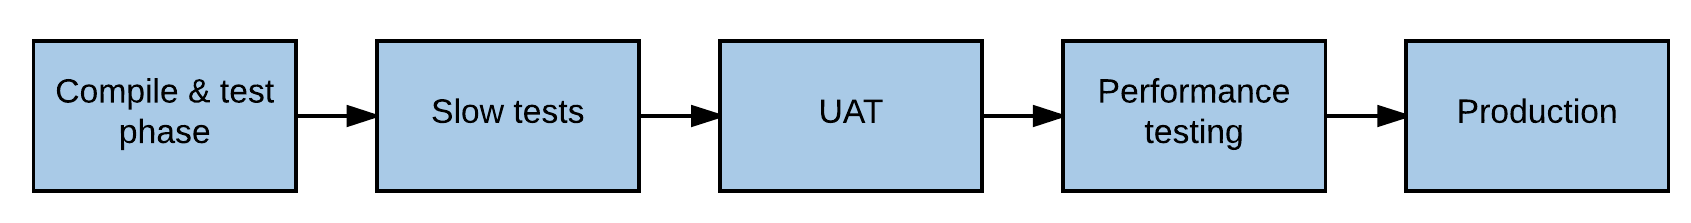
\includegraphics[scale=0.8]{architecture_microservice_build_pipeline}  
  \caption{Build pipeline(lend from Sam Newmann)}
  \label{fig:architecture_microservice_build_pipeline}
\end{figure}

\note{
Making sure that newly developed software is working is crucial. 
Being able to release microservices independently is one of the major advantages with the architecture. 
Automatic test and release of newly developed code is

\textbf{Design for failure}\\
As a consequence of partitioning the application into several service, the application needs to be designed so it can tolerate failure of entire services.


The thought of microservies is not new. But the accessibility and knowledge sharing is.

\url{https://www.youtube.com/watch?v=bHqRxMwfrng}

Monolith:
Typically kind of bad, as they grow and get more and more unmaintainable the cost of maintenance outpases the outweighs the benefits. Implementing a new feature takes a long time.

Mircroservices:
Domain driven design, understand what you are building. Break apart your business functions around bounded context, a bounded context per service.

Principals

\begin{itemize}
\item Encapsulation
\item Automation
\item Domain centric
\item Decentralized
\item Independent
\item Fail-safe
\item Observable
\end{itemize}

Scalability 

Shift to maintainability. Writing fine grained very focused micro services. It is modular, easier readable, understandable.

'Sea change' - Time is ripe. Automation, containers, Dev-Ops, higher level abstraction.

Team structure should usually be a holistic end to end team QA, product management, developers, release engineers, working together front to end. They own the product, service and so on. Ties the team together.

Partitioning strategy Verb or use-case, noun or resource, grouping things that change together. Single responsibility principle.

Benefits. Faster deployment. Easier to test. Scalability.

Challenges.
More complexity. System testing. Distributed transactions, (eventual consistency). Management of system.
Organization and culture, maturity.

Netflix
\url{https://www.youtube.com/watch?v=57UK46qfBLY}
Microservice failure
\begin{itemize}
\item Hystrix
\item Chaos monkey
\item Fault-injection test framework
\end{itemize}

}